
\section{Representations}
\subsection{Classification}
\begin{frame}[t]{Purpose}

\begin{tikzpicture}

% % always
\node (ds) at (5,0){};
\node (dsy) at (5,4){};
\node (dsx) at (10,0){};
\node (lab1) at (1,-1){\textbf{Chemical Space $C_f$}};
\foreach \x in {0,1,2}
		\foreach \y in {1,2,3}{
		\node[rectangle,fill=teal,minimum width = 0.05cm] (place\x\y) at (\x,\y){};}
% % two
\visible<2->{\node[draw,circle,very thick,red,minimum width = 0.5cm,label=right:{\color{red}$c_i$}] (ci) at (1,3){};}

% % three
\visible<1->{\node[circle, black,thick,minimum width = 2.7cm,minimum height = 2.7cm,path picture={\node at (path picture bounding box.center){\includegraphics[width=7.5cm]{representations/images/misc}}; }] (Ap) at (3.45,3.75) {};}
\visible<1->{\node (A) at (3.45,3.75) {};}
\visible<1->{\node[draw,circle,very thick,red,minimum width = 2.75cm] (cic) at (3.45,3.75){};}
\visible<1->{\path[draw,red,dashed,very thick] (ci.north) edge node[below] {} (cic.north west);}
\visible<1->{\path[draw,red,dashed,very thick] (ci.south) edge node[below] {} (cic.south);}

% % four
\visible<1->{\path[draw,very thick] (ds.center) -- (dsx);}
\visible<1->{\path[draw,very thick] (ds.center) -- (dsy);}
\visible<1->{\node (lab1) at (7,-1){\textbf{Descriptor Space $\mathcal{X}\subset \mathbb{R}^{d}$}};}

% % five
\visible<1->{\node[circle, fill=black,minimum width =0.05cm,label=below:{$\mathbf{x}_i$}] (x) at (6,3) {};}
\visible<1->{\path[draw, thick,red] (cic.north east) edge[bend left,->] node[above] {} (x);}


% % six
\visible<1->{\node[circle, fill=black,minimum width =0.05cm,label=right:{$\mathbf{x}_{j}$}] (x3) at (8,1) {};}

% % seven
\visible<1->{\node[draw,circle,very thick,red,minimum width = 0.5cm,label=below:{\color{red}$c_j$}] (cj) at (2,1){};}
\visible<1->{\node[circle, black,thick,minimum width = 2.7cm,minimum height = 2.7cm,path picture={\node at (path picture bounding box.center){\includegraphics[width=3cm]{representations/images/pisc_trans}}; }] (Xp) at (4.2,0.75) {};}
\visible<1->{\node[draw,circle,very thick,red,minimum width = 2.75cm] (cicj) at (4.2,0.75){};}
\visible<1->{\path[draw,red,dashed,very thick] (cj.north) edge node[below] {} (cicj.north west);}
\visible<1->{\path[draw,red,dashed,very thick] (cj.south) edge node[below] {} (cicj.south west);}
\visible<1->{\path[draw, thick,red] (cicj.south east) edge[bend right,->] node[below] {} (x3);}

% % eight
\visible<1->{\path[draw,dashed,gray,very thick,|-|] (x) -- (x3);}
\visible<1->{\node[gray] (ddist) at (8,2){$d(\mathbf{x}_i,\mathbf{x}_j)$};}

% %
\visible<1->{\node[align=left] (gd) at (8.2,4) {Good descriptors: \\$\bullet$ cheap \\ $\bullet$ small as possible \\ $\bullet$ preserve similarity};}


\end{tikzpicture}

\end{frame}
\begin{frame}[t]{Why similarity is important}
\tikzstyle{boxes}=[draw=black, rounded corners,very thick]
\begin{center}
{
%\fontfamily{roman}{\fontsize{10}{10}\selectfont

\begin{tikzpicture}[shorten >=1pt,draw=black!50, x = 1 in, y = 1 in,  node distance=20pt]
\draw[draw=none, use as bounding box](-0.05,-0.1) rectangle (3.295,2.85);
\node[anchor=north west,align = flush left, text width=10 cm] at (-0.5,2.85) {Different representations can have very different performance, particularly if they do not preserve notions of chemical similarity correctly:};

%\draw[help lines,step=0.82] (0,0) grid (3.3,4);


%\node [anchor=north,rotate=90] (train) at (0.001,0.4) {nearest train.};

%\node [anchor=north,rotate=90] (train) at (0.001,1.2) {Fe(II)};
%\node [anchor=north,rotate=90] (train) at (0.87,1.2) {Fe(II)};
%\node [anchor=north,rotate=90] (train) at (1.69,1.2) {Fe(II)};

\visible<2->{\node [orange]  (liex) at (1.6,1.2) {{\includegraphics[width=6.0 cm]{representations/figures/error_comp}}};}

\visible<2->{\node[text width=10cm, align=flush left] at (2,0.01){\scriptsize{{Janet, J.P., and Kulik, H.J. \textit{Chem. Sci.}, 2017, 8, 5137-5152.}}};}
\end{tikzpicture}}
\end{center}



\end{frame}
\begin{frame}[t]{Why similarity is important}
\begin{center}
\begin{tikzpicture}[shorten >=1pt,draw=black!50, x = 1 cm, y = 1cm,  node distance=20pt]
%\draw[draw=black, use as bounding box](-10,12) rectangle (10,0);
\draw[use as bounding box, anchor = north west,draw,dashed,gray] (-5.65,-3.25) rectangle (5.65,3.25);
\clip (-5.7,-3.3) rectangle (5.7,3.6);
\visible<3->{\node[rectangle, black,thick,anchor=south west] (ms1) at (-5.25,-3.25){\includegraphics[width=3.75cm]{representations/figures/split-cmes} };}
\visible<3->{\node[rectangle, black,thick,anchor=south east] (ms2) at (5.25,-3.25){\includegraphics[width=3.75cm]{representations/figures/size-cmes} };}
\visible<6->{\node[rectangle, black,thick,anchor=south west] (ms1) at (-5.25,-3.25){\includegraphics[width=3.75cm]{representations/figures/split-LS28} };}
\visible<6->{\node[rectangle, black,thick,anchor=south east] (ms2) at (5.25,-3.25){\includegraphics[width=3.75cm]{representations/figures/size-LS28} };}
%
%\visible<3->{\node[rectangle, black,thick,minimum width = 5.25cm,minimum height = 5.25cm,path picture={\node at (path picture bounding box.center){\includegraphics[width=4.5cm]{representations/figures/size-cmes}}; }] (ms1) at (5,2){};}
%
\visible<3-5>{\node (lsplit) at (-3.25,-1.0) {$\Delta E_{H-L}$};}
\visible<3-5>{\node (lsize) at (3.25,-1.0) {size};}	
	
	
\visible<1->{\node[circle,ultra thick,minimum width = 2.25 cm,minimum height =2.25 cm,draw,blue,fill opacity =0.25] (piscr) at (-4,2){};}
\visible<1->{\node[circle,minimum width = 2.25 cm,minimum height = 2.25 cm,path picture={\node at (path picture bounding box.center){\includegraphics[width=2.25cm ]{representations/images/pisc_trans.png}}; }] (piscy) at (-4,2){};}

\visible<1->{\node[rectangle,ultra thick,minimum width = 0.75 in,minimum height = 0.75 in,draw,blue,fill opacity =0.25] (miscr) at (4,2){};}

\visible<1->{\node[circle,minimum width = 2.25 cm,minimum height = 2.25 cm,path picture={\node at (path picture bounding box.center){\includegraphics[width= 4.65cm ]{representations/images/misc_trans.png}}; }] (miscyf) at (4.0,2){};}

\only<1-2>{\node[blue,anchor=north] (pisc) at (-4.0,1.0) {$\text{Fe[pisc]}_6^{3+}$};}
\only<2>{\node[blue,anchor=north] (pisc) at (4,0.40) {\footnotesize $\Delta \text{E}_{\text{H-L}}=40.7\:\text{kcal/mol}$};}
\only<1-2>{\node[blue,anchor=north] (misc) at (4.0,1.0) {$\text{Fe[misc]}_6^{3+}$};}
\only<2>{\node[blue,anchor=north] (misc) at (-4,0.40) {\footnotesize $\Delta \text{E}_{\text{H-L}}=37.7\:\text{kcal/mol}$};}
\only<5>{\path[draw,ultra thick, blue,->] (miscr.south) -- (4.80,-2.5){};}
\only<4>{\path[draw,ultra thick, blue,->] (miscr.south) -- (-1.70,-2.35){};}
\only<5>{\path[draw,ultra thick, blue,->] (piscr.south) -- (1.80,-2.65){};}
\only<4>{\path[draw,ultra thick, blue,->] (piscr.south) -- (-4.70,-2.5){};}
\end{tikzpicture}
\end{center}



\end{frame}
\begin{frame}[t]{Why similarity is important}
\begin{center}
\begin{tikzpicture}[shorten >=1pt,draw=black!50, x = 1 cm, y = 1cm,  node distance=20pt]
%\draw[draw=black, use as bounding box](-10,12) rectangle (10,0);
\draw[use as bounding box, anchor = north west,draw=none] (-5.65,-3.25) rectangle (5.65,3.25);
\clip (-5.7,-3.3) rectangle (5.7,3.6);
\node[anchor=north west,text badly centered, text width=10 cm] at (-5.5,3.2) {The richness of the representation also affects learning rate:};

\visible<2->{\node  (liex) at (0,0) {{\includegraphics[width=7.5 cm]{representations/figures/learn_rate}}};}


\end{tikzpicture}
\end{center}


\end{frame}
\begin{frame}[t]{Types of representation}
\begin{center}

\begin{tikzpicture}[x=1cm,y=1cm]
\tikzstyle{line} = [draw, -latex', very thick]
\draw[use as bounding box, anchor = north west,draw=none] (-1,-1) rectangle (5.5+4.5,3.25+2.25);
\clip (-1,-1) rectangle (10,5.5);
\linespread{0.5}
\node (ne) at (0,0) {};
\node (orig) at (-2,5) {};
\node (xe) at (10,5) {};
\node (ye) at (0,6) {};
\path [draw,very thick,->] (orig) edge node[above] {complexity}  (xe);
%\path [draw,very thick,->] (cxe) edge node[above] {cost}  (corig);
\node [rotate=90] (lab) at (-0.25,3){};
%\path [line] (orig.center)-- (ye);
\path [line] (orig.center)-- (xe);
\visible<2->{\node [draw,circle,very thick,red,fill=red,minimum width = 0.25cm,label={[align=left,below]{}}] (fpt) at (0,4) {};}
\visible<3->{\node [draw,circle,very thick,blue,fill=blue,minimum width = 0.25cm] (GGA) at (4,4) {};}
\visible<4->{\node [draw,circle,very thick,gray,fill=gray,minimum width = 0.25cm] (GGA) at (8,4) {};}
\visible<2->{\node [red] (lab1) at (0,3.25) {{Fingerprints}};}
\visible<2->{\node [align = flush left,black,text width = 3.25cm,anchor=north west] (lab13) at (-1,2.75) {\small{-- considerable use in drug design \\ $ $\\ -- no information related to molecular topology \\$ $\\ -- cheap to compute }};}
\visible<3->{\node [blue] (lab2) at (4,3.25) {Graph-theoretic};}
\visible<3->{\node [align = left,black,text width = 3.5cm,anchor=north west] (lab13) at (2.25,2.75) {\small{ -- \textit{topological}  and \textit{topochemical} representations \\ $ $\\  -- includes all connectivity but no 3D information \\ $ $\\ -- relatively easy to compute   }};}
\visible<4->{\node [align = left,gray] (lab3) at (8,3.25) {3D structure};}
\visible<4->{\node [align = left,black,text width = 3.5cm,anchor=north west] (lab13) at (5.75,2.75) {\small { -- fine-grained structural information in 3D\\ $ $\\  -- mimic input to a quantum chemistry code \\ $ $ \\ --expensive to compute, rich information}};}
\end{tikzpicture}

\end{center}

\end{frame}
\begin{frame}[t]{Ad-hoc properties}
\tikzstyle{boxes}=[draw=black, rounded corners,very thick]
\begin{center}
{
%\fontfamily{roman}{\fontsize{10}{10}\selectfont

\begin{tikzpicture}[shorten >=1pt,draw=black!50, x = 1 in, y = 1 in,  node distance=20pt]
\draw[draw=none, use as bounding box](-0.5,-0.1) rectangle (3.5,2.85);
\node[anchor=north west,align = left, text width=9.5 cm] at (-0.5,2.85) {Sometimes, simple lists of atomic propties are sufficient, especially if informed by domain knowledge:};
\visible<1->{\node (fullc) at (2.15,0.70) {\includegraphics[width=4.5 cm]{representations/images/full}};}
%\draw[help lines,step=0.82] (0,0) grid (3.3,4);


%\node [anchor=north,rotate=90] (train) at (0.001,0.4) {nearest train.};

%\node [anchor=north,rotate=90] (train) at (0.001,1.2) {Fe(II)};
%\node [anchor=north,rotate=90] (train) at (0.87,1.2) {Fe(II)};
%\node [anchor=north,rotate=90] (train) at (1.69,1.2) {Fe(II)};



\visible<2->{\node [ text width = 2.5 cm, text badly centered,red] at (0.5-0.25,2.65-0.5) {\small metal properties}{};}
\visible<3->{\node [ text width = 3 cm, text badly centered,blue] at (1.6-0.25,2.65-0.5) {\small first coord. shell}{};}
\visible<4->{\node [ text width = 3 cm, text badly centered,darkgreen] at (2.7-0.25,2.65-0.5) {\small global properties}{};}
\visible<2->{\node [trapezium,trapezium left angle=70, trapezium right angle=110, draw, ultra thick, red, minimum size = 0.7in,rounded corners] at (0.5-0.25,2.10-0.4) {};}
\visible<3->{\node [trapezium,trapezium left angle=70, trapezium right angle=110, draw, ultra thick, blue, minimum size = 0.7in,rounded corners] at (1.6-0.25,2.10-0.4) {};}
\visible<4->{\node [trapezium,trapezium left angle=70, trapezium right angle=110, draw, ultra thick, darkgreen, minimum size = 0.7in,rounded corners] at (2.7-0.25,2.10-0.4) {};}



%\foreach \x in {0.525,1.05,2.15}
%	\draw [ultra thick,black] (\x,0)--(\x,1.64);




\visible<2->{\node []  (mid) at (0.58-0.25,2.30-0.4) {\small  identity};}
\visible<2->{\node []  (oxx) at (0.425-0.25,1.90-0.4) {\small oxidation state};}
\visible<2->{\node [firebrick]  (mettxt) at (0.50-0.25,2.1-0.4) {\bf{Fe(II)}};}

\visible<3->{\node [text width = 0.75in,text badly centered]  (mid) at (1.68-0.25,2.30-0.4) {\small };}
\visible<3->{\node []  (oxx) at (1.55-0.25,1.90-0.425) {\small $\max \Delta \chi$};}
\visible<3->{\node [orange]  (liex) at (1.6-0.25,2.10-0.4) {{\includegraphics[width=0.4in]{representations/images/furanzoom}}};}
\visible<3->{\node [red]  (chiox) at (1.50-0.25,2.30-0.4) {\scriptsize $\chi = 3.44 $};}
\visible<3->{\node [gray,rectangle,fill=white,minimum height = 0.1cm,inner sep =0]  (chiC) at (1.75-0.25,2.0-0.4) {\scriptsize $\chi = 2.55 $};}

\visible<4->{\node[inner sep=0pt] (d3) at (2.68-0.25,2.18-0.4){\includegraphics[width=0.4in,angle=90]{representations/images/desc3}};}
\visible<4->{\node []  (oxx) at (2.65-0.25,1.90-0.4) {\small Kier index};}



\visible<5->{\node [anchor=south west]  (liex) at (-0.5,-0.1) {{\includegraphics[width=4 cm]{representations/figures/error_comp}}};}


%\node [orange]  (liex) at (1.5,0.75) {{\includegraphics[width=4 cm]{images/local}}};
%\node [orange]  (liex) at (1.5,0.75) {{\includegraphics[width=4 cm]{images/partial}}};
%\node [orange]  (liex) at (1.5,0.75) {{\includegraphics[width=4 cm]{images/full}}};



\visible<5->{\node[text width=5cm] at (2.20,0.125){\scriptsize{{Janet, J.P., and Kulik, H.J. \textit{Chem. Sci.}, 2017, 8, 5137-5152.}}};}
\end{tikzpicture}}
\end{center}



\end{frame}
\begin{frame}[t]{Fingerprints and the low-information limit}

In cheminformatics (esp. drug design literature) fingerprints are binary vectors used to determine molecular similarity. For example, FP2 fingerprint is a  1024 bit fingerprint:
\begin{center}
\only<2>{\includegraphics[width=5cm]{representations/images/tbb.png}}
\only<3>{\includegraphics[width=5cm]{representations/images/tb.png}}
\only<4>{\includegraphics[width=5cm]{representations/images/tbc.png}}
\end{center}




\end{frame}
\begin{frame}[t]{Molecular graphs}
Based on  autocorrelations\only<1>{\footnote{Broto, P., Moreau, G. and Vandycke, C. \textit{Eur. J. Med. Chem.}, 19(1):71-78, 1984.}}\only<2->{\setcounter{footnote}{3} and modified for TMCs}\only<2->{\footnote{Janet, J.P., and Kulik, H.J. \textit{J. Phys. Chem. A}, 2017,121, 46, 8939-8954.}}

\begin{tikzpicture}[node distance=20pt]
\tikzstyle{boxes}=[draw=red, rounded corners]
\definecolor{dist}{rgb}{0,0,0.54}
\definecolor{prox}{rgb}{0.6953125,0.1328125,0.1325125}
\definecolor{mid}{rgb}{0,0.39,0}
\tikzstyle{met} = [circle, draw, fill=blue!20,minimum size = 1.5cm, 
text width=1.25cm, text badly centered, node distance=3cm, inner sep=0pt]
\tikzstyle{graphn} = [circle, draw, thick, fill=darkgray!20,minimum size = 0.5cm, 
text width=1cm, text badly centered, node distance=3cm, inner sep=0pt]
\tikzstyle{carb} = [circle, draw, fill=gray!20,minimum size = 1cm, 
text width=1cm, text badly centered, node distance=3cm, inner sep=0pt]
\tikzstyle{ox} = [circle, draw, fill=red!20,minimum size = 0.5cm, 
text width=0.8cm, text badly centered, node distance=3cm, inner sep=0pt]  

\visible<14->{\fill[fill=dist!45]
    (-2,3) -- (-2,-2)  -- (2,-2) --(2,3);}
\visible<14->{\fill[fill=mid!45]
    (-2,3) -- (-2,-0.75)  -- (2,-0.75) --(2,3);}
\visible<14->{\fill[fill=prox!45]
    (-2,3) -- (-2,0.75)  -- (2,0.75) --(2,3);}
%%%%%%%%%%%%%%%%%%%%%%%%%%%%%%%%%%%%%5
\visible<1-17>{\node[ox] at (1.5,1.5) (ox1){O};}
\visible<1-17>{\node[ox] at (-1.5,1.5) (ox2){O};}
\visible<1-17>{\node[ox] at (1.5,-1.5) (ox3){O};}
\visible<1-17>{\node[ox] at (-1.5,-1.5) (ox4){O};}
\visible<1-17>{\node[carb] at (-0.75,0) (c1){C};}
\visible<1-17>{\node[carb] at (0.75,0) (c2){C};}
\visible<8-17>{\node[met] at (0,3) (m){M};}
\visible<1-17>{\path[draw, very thick] (ox1) -- (c2){};}
\visible<1-17>{\path[draw, very thick] (ox2) -- (c1){};}
\visible<1-17>{\path[draw, very thick] (ox3) -- (c2){};}
\visible<1-17>{\path[draw, very thick] (ox4) -- (c1){};}
\visible<1-17>{\path[draw, very thick] (c2) -- (c1){};}
\visible<1-17>{\path[draw, very thick] (c2) -- (c1){};}
\visible<8-17>{\path[draw,dashed, very thick] (m) -- (ox1){};}
\visible<8-17>{\path[draw,dashed, very thick] (m) -- (ox2){};}

%%%%%%%%%%%%%%%%%%%%%%%%%%%%%%%%%%%%%5 
\visible<2-4>{\node[fill  = orange!50,draw = red, ultra thick, fill opacity = 0.15,rounded corners,rectangle,minimum size=1.25cm] at (ox2.center){};}
\visible<3-4>{\node[fill  = blue!50,draw = blue,dashed, ultra thick, fill opacity = 0.05,rounded corners,rectangle,minimum size=1.05cm,rotate = 45] at (c1.center){};}
\visible<3-4>{\path[draw, ultra thick] (ox2.center) edge[bend left,blue,->] (c1.center);}
\visible<4>{\node[anchor = west] (eq) at (2.0,1.5){\small $\begin{aligned} \color{blue}d_1\color{black} : \sum_{\color{red}{O}\color{black},\color{gray}{C}}\color{black} Z_{O}Z_{C} = 48\end {aligned}$};}

\visible<5>{\node[fill  = orange!50,draw = red, ultra thick, fill opacity = 0.15,rounded corners,rectangle,minimum size=1.25cm] at (c1.center){};}
\visible<5>{\node[fill  = blue!50,draw = blue,dashed, ultra thick, fill opacity = 0.05,rounded corners,rectangle,minimum size=1.05cm,rotate = 45] at (ox2.center){};}
\visible<5>{\node[fill  = blue!50,draw = blue,dashed, ultra thick, fill opacity = 0.05,rounded corners,rectangle,minimum size=1.05cm,rotate = 45] at (ox4.center){};}
\visible<5>{\node[fill  = blue!50,draw = blue,dashed, ultra thick, fill opacity = 0.05,rounded corners,rectangle,minimum size=1.05cm,rotate = 45] at (c2.center){};}
\visible<5>{\node[anchor = west] (eq) at (2.0,1.5){\small $\begin{aligned} \color{blue}d_1\color{black} : 48 +  \sum_{\color{gray}{C}\color{black},\color{red}{O}}\color{black} Z_{O}Z_{C} = 144 + 48\end {aligned}$};}
\visible<5>{\path[draw, ultra thick] (c1.center) edge[bend left,blue,->] (c2.center);}
\visible<5>{\path[draw, ultra thick] (c1.center) edge[bend left,blue,->] (ox2.center);}
\visible<5>{\path[draw, ultra thick] (c1.center) edge[bend right,blue,->] (ox4.center);}


\visible<6>{\node[fill  = orange!50,draw = red, ultra thick, fill opacity = 0.15,rounded corners,rectangle,minimum size=1.25cm] at (c1.center){};}
\visible<6>{\node[fill  = orange!50,draw = red, ultra thick, fill opacity = 0.15,rounded corners,rectangle,minimum size=1.25cm] at (c2.center){};}
\visible<6>{\node[fill  = orange!50,draw = red, ultra thick, fill opacity = 0.15,rounded corners,rectangle,minimum size=1.25cm] at (ox1.center){};}
\visible<6>{\node[fill  = orange!50,draw = red, ultra thick, fill opacity = 0.15,rounded corners,rectangle,minimum size=1.25cm] at (ox2.center){};}
\visible<6>{\node[fill  = orange!50,draw = red, ultra thick, fill opacity = 0.15,rounded corners,rectangle,minimum size=1.25cm] at (ox3.center){};}
\visible<6>{\node[fill  = orange!50,draw = red, ultra thick, fill opacity = 0.15,rounded corners,rectangle,minimum size=1.25cm] at (ox4.center){};}
\visible<6>{\node[anchor = west] (eq) at (2.15,1.5){\small $\begin{aligned} \color{blue}d_1\color{black} : \sum_{i}\sum_{j}\color{black} Z_{i}Z_{j} \delta (d_{i,j},\color{blue}1\color{black}) \end {aligned}$};}
\visible<7>{\node[anchor = west] (eq) at (2.15,1.5){\small $\begin{aligned} \color{blue}d_x\color{black} : \sum_{i}\sum_{j}\color{black} Z_{i}Z_{j} \delta (d_{ij},\color{blue}x\color{black}) \end {aligned}$};}



%%%%%%%%%%%%%%%%%%%%%%%%%%%%%%%%%%%%%%%%%
%%%%%%%%%%%%%%%%%%%%%%%%%%%%%%%%%%%%%%%%%


\visible<7>{\node[anchor = west] (eq) at (2.15,-0.5){\includegraphics[width= 5.25cm]{representations/figures/ACD}};}


%%%%%%%%%%%%%%%%%%%%%%%%%%%%%%%%%%%%%%%%%
\visible<8->{\node[anchor = west] (eq) at (2.15,1.5){\small How to adapt to TM complexes?};}
\visible<9->{\node[anchor = west,align = left] (eq) at (2.15,0.80){\small restrict the scope to focus on \\ \small \textit{near-metal atoms}};}
%%%%%%%%%%%%%%%%%%%%%%%%%%%%%%%%%%%%%%%%%
\visible<10-12>{\node[fill  = orange!50,draw = red, ultra thick, fill opacity = 0.15,rounded corners,rectangle,minimum size=1.25cm] at (m.center){};}
\visible<11>{\node[fill  = blue!50,draw = blue,dashed, ultra thick, fill opacity = 0.05,rounded corners,rectangle,minimum size=1.05cm,rotate = 45] at (ox1.center){};}
\visible<11>{\node[fill  = blue!50,draw = blue,dashed, ultra thick, fill opacity = 0.05,rounded corners,rectangle,minimum size=1.05cm,rotate = 45] at (ox2.center){};}

\visible<11>{\path[draw, ultra thick,blue] (ox1.center) edge [bend right,<-] node {} (m.center){};}
\visible<11>{\path[draw, ultra thick,blue] (ox2.center) edge [bend left,<-] node {} (m.center){};}

\visible<11>{\node[anchor = west] (eq) at (2.0,-0.25){\small $\begin{aligned} \color{blue}d_1\color{black} : \sum_{\color{blue!50}{M}\color{black},\color{red}{O}} Z_{M}Z_O \end{aligned}$};}
%\visible<16>{\node[rectangle,minimum width = 1cm,black] (vectc1) at (-3,2){112};}

\visible<12>{\node[fill  = blue!50,draw = blue,dashed, ultra thick, fill opacity = 0.05,rounded corners,rectangle,minimum size=1.05cm,rotate = 45] at (c1.center){};}
\visible<12>{\node[fill  = blue!50,draw = blue,dashed, ultra thick, fill opacity = 0.05,rounded corners,rectangle,minimum size=1.05cm,rotate = 45] at (c2.center){};}

\visible<12>{\path[draw, ultra thick,blue] (c1.center) edge [bend left,<-] node {} (m.center){};}
\visible<12>{\path[draw, ultra thick,blue] (c2.center) edge [bend right,<-] node {} (m.center){};}

\visible<12>{\node[anchor = west] (eq) at (2.0,-0.25){\small $\begin{aligned} \color{blue}d_2\color{black} : \sum_{\color{blue!50}{M}\color{black},\color{gray}{C}} Z_{M}Z_C  \end{aligned}$};}


%%%%%%%%%%%%%%%%%%%%%%%%%%%%%%%55

\visible<13>{\node[fill  = blue!50,draw = blue,dashed, ultra thick, fill opacity = 0.05,rounded corners,rectangle,minimum size=1.05cm,rotate = 45] at (ox3.center){};}
\visible<13>{\node[fill  = blue!50,draw = blue,dashed, ultra thick, fill opacity = 0.05,rounded corners,rectangle,minimum size=1.05cm,rotate = 45] at (ox4.center){};}

\visible<13>{\path[draw, ultra thick,blue] (ox3.center) edge [bend right,<-] node {} (m.center){};}
\visible<13>{\path[draw, ultra thick,blue] (ox4.center) edge [bend left,<-] node {} (m.center){};}

\visible<13->{\node[anchor = west] (eq) at (2.0,-0.25){\small $\begin{aligned} \color{blue}d_3\color{black} : \sum_{\color{blue!50}{M}\color{black},\color{red}{O}} Z_{M}Z_O  \end{aligned}$};}






%%%%%%%%%%%%%%%%%%%%%%%%%%%%%%%%%%%%%%%%%
%\visible<13->{\node[fill  = orange!50,draw = red, ultra thick, fill opacity = 0.15,rounded corners,rectangle,minimum size=1.25cm] at (ox1.center){};}
%\visible<13->{\node[fill  = orange!50,draw = red, ultra thick, fill opacity = 0.15,rounded corners,rectangle,minimum size=1.25cm] at (ox2.center){};}
%
%\visible<13->{\node[anchor = west] (eq) at (2,-0.15){\small $\begin{aligned} \color{blue}d
%\color{black} : \frac{1}{\left\vert lc \right\vert}\sum_{i\in lc}\sum_{j} Z_iZ_j \delta (d_{ij}, 
%\color{blue}d\color{black}) \end{aligned}$};}%%


\visible<15->{\node[anchor = west,red, ultra thick] (neq) at (3,-1) {$
\color{red}\left(Z_i - Z_j\right)\color{black} $};}
\visible<16>{\node[anchor = west,rectangle,ultra thick] (neq) at (3,-1.75) {properties:$\color{black}T\color{black}$,$\color{black}\chi\color{black}$,$\color{black}Z\color{black}$,$\color{black}I\color{black}$,$\color{black}S\color{black}$ };}
\visible<17->{\node[anchor = west,rectangle,draw, ultra thick] (neq) at (4,-1.75) {\small $\sim 160$ features in total};}


%%%%%%%%%%%%%%%%%%%%%%%%%%%%%%%%%%%%%%%%%
\end{tikzpicture}
\end{frame}

\begin{frame}[t]{Coulomb matrices}
\begin{center}
\begin{tikzpicture}[x=1cm,y=1cm]
%\pgfresetboundingbox
\draw[use as bounding box, anchor = north west,draw=none] (-5.5,-3.25) rectangle (5.5,3.25);
\clip (-5.5,-3.25) rectangle (5.5,3.25);
\only<1->{\node[anchor =north west] (text) at (-5.25,3.25){\begin{minipage}{10.0cm}
One family of 3D desciptors attempt to copy information used in quantum chemistry codes, e.g. Coulomb Matricies:\\
\scriptsize  Montavon, G. \textit{et al.}. Learning Invariant Representations of Molecules for Atomization Energy Prediction, NIPS 25, 2012 \normalsize
\begin{align*}
M_{I,J} = 
\begin{cases}
0.5Z_{I}^{2.4}& \text{for } I = J \\
\frac{Z_{I}Z_{J}}{|R_I-R_J|}&  \text{for } I \neq J
\end{cases}
\end{align*}		
\end{minipage}};}
\visible<1->{\node[anchor=east] (east) at (3.5,-1.5){\includegraphics[width=3.5cm]{representations/images/coulomb_matrix_performance.png}};}
\visible<1->{\node[anchor=west] (figure) at (-4.5,-1.5){\includegraphics[width=3.5cm]{representations/images/coulomb_matrix.png}};}
\only<2->{\node[anchor = south] (text) at (1.5,-3.25){\begin{minipage}{10.0cm}
rotational and translational invariance
\end{minipage}};}
\end{tikzpicture}
\end{center}

\end{frame}
\begin{frame}[t]{HDAD and beyond-CM}
Descriptors derived from geometric parameters, i.e. bonds, angles, and dihedral angles:
\begin{align*}
\includegraphics[width=1cm]{representations/images/HDAD.jpg}
\includegraphics[width=3cm]{representations/images/HDAD_performance.jpg}
the red and blue lines were trained with Laplacian and Guassian kernels, respectively.
\end{align*}

\end{frame}

\begin{frame}[t]{System and atom level features}
\begin{center}

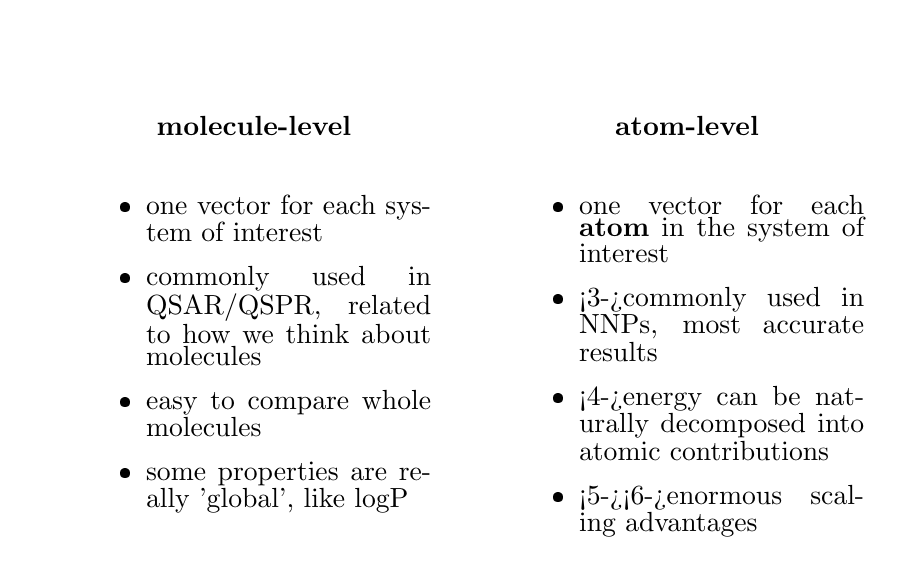
\begin{tikzpicture}[x=1cm,y=1cm]
\tikzstyle{line} = [draw, -latex', very thick]
\draw[use as bounding box, anchor = north west,draw=none] (-1,-1) rectangle (5.5+4.5,3.25+2.25);
\clip (-1,-1) rectangle (10,5.5);
\linespread{0.5}
%\path [draw,very thick,->] (cxe) edge node[above] {cost}  (corig);
\visible<1->{\node [text badly centered,black,text width = 4.5cm,anchor=north west] (lab13) at (-0.5,4.5) {\textbf{molecule-level}};}

\visible<1->{\node [align = flush left,black,text width = 3.25cm,anchor=north west] (lab13) at (-0.5,3.5) {
		\begin{minipage}{4.5cm}
		\begin{itemize}
		\item one vector for each system of interest
		\item commonly used in QSAR/QSPR, related to how we think about molecules
		\item easy to compare whole molecules
		\item some properties are really 'global', like logP
		\end{itemize}
		\end{minipage}};}
\visible<2->{\node [text badly centered,black,text width = 4.5cm,anchor=north west] (lab13) at (5,4.5) {\textbf{atom-level}};}
\visible<2->{\node [align = flush left,black,text width = 3.25cm,anchor=north west] (lab13) at (5,3.5) {
		\begin{minipage}{4.5cm}
		\begin{itemize}
		\item one vector for each \textbf{atom} in the system of interest
		\item \visible<3->{commonly used in NNPs, most accurate results}
		\item \visible<4->{energy can be naturally decomposed into atomic contributions}
		\item \visible<5->{\only<6->{\color{red}}enormous scaling advantages}
		\end{itemize}
		\end{minipage}};}

\end{tikzpicture}

\end{center}

\end{frame}

\begin{frame}[t]{System and atom level features}
\begin{center}

\begin{tikzpicture}[x=1cm,y=1cm]
\tikzstyle{line} = [draw, -latex', very thick]
\draw[use as bounding box, anchor = north west,draw=none] (-1,-1) rectangle (5.5+4.5,3.25+2.25);
%\clip (-1,-1) rectangle (10,5.5);
\linespread{0.5}
%\path [draw,very thick,->] (cxe) edge node[above] {cost}  (corig);
\only<1->{\node[anchor =north west] (text) at (-0.5,5.75){\begin{minipage}{10.0cm}
		Basic idea is to create an atomic level represenstation that `knows' about the neighborhood:\\
		\scriptsize  J. Behler. First Principles Neural Network Potentials for Reactive Simulations of Large Molecular and Condensed Systems, \textit{Angew. Chem. Int. Ed.}, 56, 12828, 2017 \normalsize
		\end{minipage}};}
\visible<2->{\node[anchor=west] (im1) at (-0.5,1.5){\includegraphics[width=3.5cm]{representations/images/behler-sym-0.png}};}
\visible<3->{\node[anchor=west] (im2) at (5.5,1.5){\includegraphics[width=3.15cm]{representations/images/behler-sym-1.png}};}
\visible<3->{\path[draw,blue,ultra thick,->] (im1) -- (im2);}
\visible<4->{\node[anchor =north west, blue] (text) at (-0.5,-0.15){\begin{minipage}{5.5cm}
		\scriptsize  J. Behler and M. Parrinello. Generalized Neural-Network Representation of High-Dimensional Potential-Energy Surfaces, \textit{Phys. Rev. Lett.}, 98, 146401, 2007
		\end{minipage}};}

\end{tikzpicture}

\end{center}

\end{frame}

\begin{frame}[t]{Learning representations}
\begin{center}

\begin{tikzpicture}[x=1cm,y=1cm]
\tikzstyle{line} = [draw, -latex', very thick]
\draw[use as bounding box, anchor = north west,draw=none] (-1,-1) rectangle (5.5+4.5,3.25+2.25);
%\clip (-1,-1) rectangle (10,5.5);
\linespread{0.5}
%\path [draw,very thick,->] (cxe) edge node[above] {cost}  (corig);
\only<1->{\node[anchor =north west] (text) at (-0.5,5.75){\begin{minipage}{10.0cm}
		We can directly learn what features to have using NNs  -- graph convolutions (more on this in NN section)\\
		\scriptsize Duvenaud, D. \textit{et al.}.Convolutional Networks on Graphs
		for Learning Molecular Fingerprints, NIPS 28, 2015 \normalsize
		\end{minipage}};}
\visible<2->{\node[anchor=west] (im1) at (-0.5,1.0){\includegraphics[width=9.5cm]{representations/images/gc1.png}};}
\visible<3->{\node[anchor=west] (im2) at (4.0,3.5){\includegraphics[width=5.5cm]{representations/images/gc2.png}};}
\end{tikzpicture}

\end{center}

\end{frame}

\begin{frame}[t]{Conclusions}
In summary:
\vspace{1cm}
\pause{}
\begin{enumerate}
	\item Different encoding schemes use different amounts of information \pause{}
	\item The representation needs to matched to the application in question \pause{}
	\item Feature selection techniques can help identify important features, for modeling and for interpretation
\end{enumerate}

\end{frame}
